\chapter{Line Mode} 
\label{sec:linemode}
\lstset{style=6502Style}

\begin{figure}[H]
    \centering
    \begin{adjustbox}{width=10.5cm,margin=0cm}
      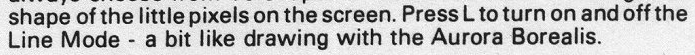
\includegraphics[width=12cm]{src/linewidth/linemode.png}%
    \end{adjustbox}
    \caption{
      Excerpt from Manual (Part No. LC1982-Vb). Line Width.
      }
\end{figure}

\begin{figure}[H]
    \centering
    \begin{adjustbox}{width=10.5cm,margin=0cm}
      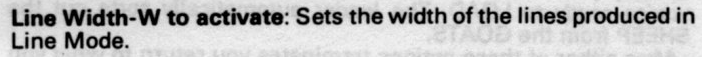
\includegraphics[width=12cm]{src/linewidth/linewidth.png}%
    \end{adjustbox}
    \caption{
      Excerpt from Manual (Part No. LC1982-Vb). Line Width.
      }
\end{figure}

\begin{figure}[H]
    \centering
    \foreach \l in {0,...,10}
    {
      \includegraphics[width=4.2cm]{linewidth/pattern\l-45.png}%
    }%
    \caption{
      Line Mode with Pulse Width at Maximum
      }
\end{figure}
\clearpage

\begin{figure}[H]
    \centering
    \foreach \l in {0,...,10}
    {
      \includegraphics[width=4.2cm]{linewidth/pattern1-\l-45.png}%
    }%
    \caption{
      Line Mode with Pulse Width at Minimum
      }
\end{figure}
\clearpage

\clearpage
\begin{lstlisting}[caption=From \icode{MainInterruptHandler}.]
        ; Line Mode Active
        LDA #$19
        SEC 
        SBC colorRAMLineTableIndex
        ORA #$80
        STA currentIndexForCurrentStepArray,X
\end{lstlisting}

\begin{lstlisting}[caption=From \icode{MainPaintLoop}.]
        ; Line Mode sets the top bit of currentIndexToColorValues
        LDA currentIndexToColorValues
        AND #$80
        BNE PaintLineModeAndLoop
        ...
PaintLineModeAndLoop
        ; Loops back to MainPaintLoop
        JMP PaintLineMode
\end{lstlisting}

\clearpage

\textbf{Lines 1189-1231. \icode{\textbf{DisplayPresetMessage}}:} 
\clearpage

\clearpage
\begin{lstlisting}[caption=From \icode{PaintLineMode}.]
PaintLineMode 
        LDA currentIndexToColorValues
        AND #$7F
        STA offsetForYPos
        LDA #$19
        SEC 
        SBC offsetForYPos
        STA pixelYPositionZP
        DEC pixelYPositionZP
        LDA #$00
        STA currentIndexToColorValues
        LDA #$01
        STA skipPixel
        JSR PaintPixelForCurrentSymmetry
        INC pixelYPositionZP
        LDA #$00
        STA skipPixel

        LDA lineWidth
        EOR #$07
        STA currentIndexToColorValues
LineModeLoop   
        JSR PaintPixelForCurrentSymmetry
        INC pixelYPositionZP
        INC currentIndexToColorValues
        LDA currentIndexToColorValues
        CMP #$08
        BNE ResetLineModeColorValue
        JMP CleanUpAndExitLineModePaint

        INC currentIndexToColorValues
ResetLineModeColorValue   
        STA currentIndexToColorValues
        LDA pixelYPositionZP
        CMP #$19
        BNE LineModeLoop

CleanUpAndExitLineModePaint    
        LDX currentBufferLength
        DEC currentIndexForCurrentStepArray,X
        LDA currentIndexForCurrentStepArray,X
        CMP #$80
        BEQ ResetIndexAndExitLineModePaint
        JMP MainPaintLoop

ResetIndexAndExitLineModePaint   
        LDA #$FF
        STA currentIndexForCurrentStepArray,X
        STX shouldDrawCursor
        JMP MainPaintLoop
\end{lstlisting}
\clearpage

\textbf{Lines 1189-1231. \icode{\textbf{DisplayPresetMessage}}:} 
\clearpage
